%%
%% GAC: When Smaller Is Slower — Dimensional Misalignment in Compressed LLMs
%% Target: EuroMLSys 2026 (SIGPLAN format, 6 pages excluding references)
%%

\documentclass[sigplan,10pt,nonacm]{acmart}

%% Remove ACM-specific elements for submission
\settopmatter{printacmref=false,authorsperrow=5}
\renewcommand\footnotetextcopyrightpermission[1]{}
\pagestyle{plain}

%% Packages
\usepackage{booktabs}
\usepackage{subcaption}
\usepackage{xcolor}
\usepackage{graphicx}
\usepackage{tikz}
\usetikzlibrary{positioning,decorations.pathreplacing,fit,backgrounds}
\usepackage{placeins}
\usepackage{colortbl}
\usepackage{enumitem}
\hfuzz=0pt  % Strict: report ALL overfull boxes

%% Compact spacing
\setlength{\textfloatsep}{8pt plus 2pt minus 2pt}
\setlength{\floatsep}{8pt plus 2pt minus 2pt}
\setlength{\intextsep}{6pt plus 2pt minus 2pt}
\setlength{\abovecaptionskip}{4pt}
\setlength{\belowcaptionskip}{2pt}

%% Colors matching slides
\definecolor{cblue}{RGB}{55,131,187}
\definecolor{cred}{RGB}{211,63,73}
\definecolor{cgreen}{RGB}{56,158,92}
\definecolor{corange}{RGB}{230,159,0}

%% Title
\title{Why Smaller Is Slower?\\ Dimensional Misalignment in Compressed LLMs}

%% Authors
\author{Jihao Xin}
\affiliation{
  \institution{KAUST}
  \country{Saudi Arabia}
}

\author{Tian Lyu}
\affiliation{
  \institution{KAUST}
  \country{Saudi Arabia}
}

\author{Qilong Pan}
\affiliation{
  \institution{HUMAIN AI}
  \country{Saudi Arabia}
}

\author{Kesen Wang}
\affiliation{
  \institution{HUMAIN AI}
  \country{Saudi Arabia}
}

\author{Marco Canini}
\affiliation{
  \institution{KAUST}
  \country{Saudi Arabia}
}

\begin{abstract}
Post-training compression reduces LLM parameter counts but often produces irregular tensor dimensions that degrade GPU performance---a phenomenon we call \emph{dimensional misalignment}.
We present a full-stack analysis of this effect, identifying root causes at three levels: framework (PyTorch backend dispatch), library (cuBLAS kernel selection), and hardware (TensorCore and memory alignment).
We propose \textbf{GAC} (GPU-Aligned Compression), a general framework that wraps any compressor and selects GPU-Aligned dimensions via multi-choice knapsack optimization.
On Llama-3-8B with two representative compressors---ASVD (SVD factorization) and LLM-Pruner (structured pruning)---GAC achieves 100\% dimension alignment with up to 1.5$\times$ speedup while preserving model quality.
\end{abstract}

\keywords{LLM Compression, GPU Optimization}

\begin{document}

\maketitle


%% ===========================================
%% 1. INTRODUCTION
%% ===========================================
\section{Introduction}
\label{sec:intro}

Large Language Models (LLMs) achieve strong capabilities but their scale poses deployment challenges~\cite{llama3}.
Post-training compression reduces model size which can be categorized into three categories: \emph{quantization} (reduced precision)~\cite{gptq,awq}, \emph{sparsification} (zeroing weights)~\cite{sparsegpt,wanda}, and \emph{dimension reduction} (low-rank factorization, structured pruning, KV cache eviction)~\cite{asvd,palu,llmpruner,h2o,pyramidkv}.
We focus on \textbf{dimension reduction}: it alters the tensor shapes that feed the dominant inference operators, which often produce \emph{irregular} dimensions (e.g., reduced rank from 128 to 107), which is inefficient in GPU's execution, and leads to a counterintuitive outcome: \emph{compressed models with \textbf{smaller} parameters can run \textbf{slower} than uncompressed models}. We term this \textbf{dimensional misalignment}.
We summarize three classes of compression algorithms that lead to dimensional misalignment: \textbf{(i)}~low-rank factorization (decomposing weight matrices into two smaller matrices $W \approx A \cdot B$, truncating inner dimension),~\cite{asvd,palu,svdllm2024}; \textbf{(ii)}~structured pruning (removing neurons or heads, reducing output dimension),~\cite{llmpruner,sparsegpt,wanda}; \textbf{(iii)}~token eviction (dropping or compressing keys/values, reducing effective sequence length),~\cite{h2o,pyramidkv}.

Existing compression methods predominantly trade off \emph{size and accuracy}: given a compression ratio, they maximize preserved accuracy while ignoring how chosen dimensions interact with hardware.
We propose \textbf{GAC} (GPU-Aligned Compression), a new compression \emph{paradigm} that imposes hardware alignment constraints on top of existing dimension-reducing compressors: it wraps any such compressor and selects hardware-aligned dimensions under the same parameter budget, restoring speed without changing the compressor's accuracy-oriented design.

\noindent \textbf{Contributions.}\\
\textbf{(1)}~We identify the \emph{dimensional misalignment} problem (\S\ref{sec:misalignment}).\\
\textbf{(2)}~We conduct a systematic full-stack analysis (\S\ref{sec:analysis}).\\
\textbf{(3)}~GAC formalizes the dimension selection as a constrained optimization with a dynamic programming solver (\S\ref{sec:gac}).\\
\textbf{(4)}~Preliminary evaluation on Llama-3-8B shows up to 1.5$\times$ speedup (\S\ref{sec:eval}).


%% ===========================================
%% 2. DIMENSIONAL MISALIGNMENT
%% ===========================================
\section{Dimensional Misalignment}
\label{sec:misalignment}
\begin{figure*}[t]
  \centering
  \includegraphics[width=\textwidth]{figures/scatter_1x4_meta_llama_3_8b_instruct_r0.8.pdf}
  \caption{Llama-3-8B at $\rho=20\%$. Shape: $\circ{=}$Q Head, $\square{=}$K Head, $\triangle{=}$V Head; color: \textcolor{cgreen}{green}=8-aligned, \textcolor{cred}{red}=misaligned.}
  \label{fig:dim_scatter}
  \end{figure*}
    
Existing LLM compression aims to preserve accuracy under a given compression ratio $\rho$.
Formally, given the set of pretrained parameters $\mathcal{W}$, we seek a compressed set $\mathcal{W}'$ that minimizes expected loss subject to the size constraint:
\begin{equation}
\min_{\mathcal{W}'} \; \mathbb{E}_{(x,y)\sim\mathcal{D}}[\mathcal{L}(\mathcal{W}'; x, y)] \quad \text{s.t.} \quad 1-|\mathcal{W}'|/|\mathcal{W}| \leq \rho.
\label{eq:compression_target}
\end{equation}
Here $\mathcal{D}$ is the data distribution, $\mathcal{L}$ is the loss, $|\mathcal{W}'|$ and $|\mathcal{W}|$ denote total parameter counts. We denote $B = (1-\rho)|\mathcal{W}|$ as the parameter budget.

Different parameters have different compression sensitivities, e.g., early and late layers are often more critical than middle layers---so budget cannot be allocated uniformly.
Existing methods proceed in two steps.
First, for each parameter $W_i$, compute an \textbf{importance score} $s_i$ using a proxy (Table~\ref{tab:importance_scores}); a higher $s_i$ reflects higher sensitivity thus should retain more parameters in $W_i$.
Second, allocate the budget $B$ by assigning each $W_i$ a dimension $d_i$ thus that more important $W_i$ receive larger $d_i$:
\begin{equation}
\{d_i\} = \arg\max_{\{d_i\}} \sum_i s_i \cdot |W_i| \quad \text{s.t.} \quad |\mathcal{W}'| \leq B, \quad d_i \geq 0.
\label{eq:budget_allocation}
\end{equation}
Here $d_i$ is the compressed dimension (e.g., inner rank or output width, varies by compression method), $|W_i|$ is the parameter count given dimension $d_i$, $|\mathcal{W}'| = \sum_i |W_i|$ is the total parameter count of the compressed model, and $B$ is the parameter budget.
Because $s_i$ and the optimum $\{d_i\}$ are continuous, the resulting dimensions are typically \emph{irregular} (e.g., 107, 108, 109) and often violate GPU alignment requirements (e.g.\ $d \bmod 8 = 0$), triggering backend fallbacks and kernel switches that erase the expected speedup from fewer parameters and FLOPs.

We demonstrate the dimensional misalignment problem with a real-world example: PaLU~\cite{palu}.
We use \textbf{8-alignment} ($d \bmod 8 = 0$) as an example of alignment constraints. When dimensions are not 8-aligned, latency can increase by up to 90\% (Figure~\ref{fig:sdpa_latency}); we detail this analysis in \S\ref{sec:analysis}.
Figure~\ref{fig:palu_dist} shows that a large fraction of layers end up misaligned (e.g., 78\% in this setup).
For generality, we summarize the mainstream importance score proxies into four categories (Table~\ref{tab:importance_scores}).
We empirically measure unconstrained dimension allocation on Llama-3-8B at $\rho=20\%$ with all four proxies, Figure~\ref{fig:dim_scatter} demonstrates the dimensional misalignment consistently occurs across different methods.
\begin{figure}[t]
\centering
\includegraphics[width=\columnwidth]{figures/fig3_palu_dist.png}
\caption{Llama-3-8B after PaLU compression at $\rho=20\%$.}
\label{fig:palu_dist}
\end{figure}

\begin{table}[t]
\centering
\caption{Mainstream importance score for budget allocation.}
\label{tab:importance_scores}
\small
\setlength{\tabcolsep}{4pt}
\begin{tabular}{@{}llll@{}}
\toprule
\textbf{Method} & \textbf{Score} & \textbf{Intuition} & \textbf{Works} \\
\midrule
Magnitude & $\|W_i\|_F$ & Weight norm & SVD-LLM~\cite{svdllm2024} \\
Activation & $\|X_i\|_F$ & Input magnitude & ASVD~\cite{asvd} \\
Gradient & $\left|\frac{\partial \mathcal{L}}{\partial h_i} \cdot h_i\right|$ & Taylor expansion & Taylor Pruning~\cite{taylor_pruning} \\
Fisher & $\mathrm{tr}(\mathbf{F}_i)$ & Curvature of loss & PaLU~\cite{palu}, FWSVD~\cite{fwsvd2022} \\
\bottomrule
\end{tabular}
\end{table}


%% ===========================================
%% 3. FULL-STACK ANALYSIS
%% ===========================================

\section{Full-Stack Analysis}
\label{sec:analysis}
We analyze where and why dimensional misalignment causes slowdowns on an NVIDIA A100-80GB with PyTorch 2.9.1, CUDA 12.8, FP16.
Latency is measured with CUDA events (50 warmup, 200 measurement iterations, 3 trials).
Root causes fall into three layers (Figure~\ref{fig:fullstack_overview}): Framework, Library, and Hardware. We detail each layer in the following subsections.
\begin{figure}[t]
  \centering
  \resizebox{\columnwidth}{!}{%
  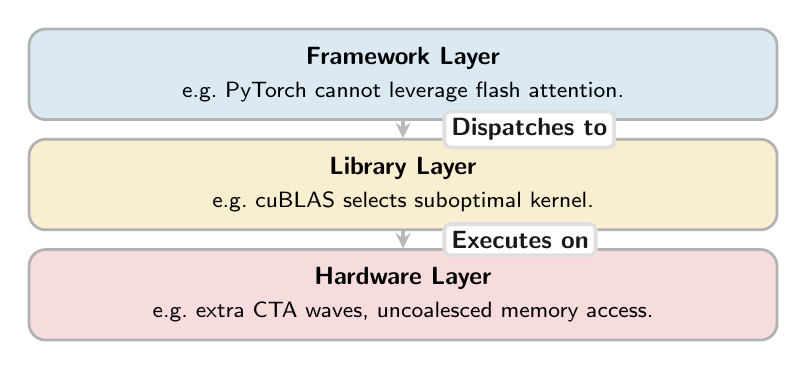
\begin{tikzpicture}[
      layer/.style={draw=gray!60, rounded corners=6pt, minimum width=9.5cm, minimum height=1.15cm,
                    line width=1pt, font=\sffamily\small, align=center, inner sep=6pt},
      >=stealth, arrow/.style={->, line width=1.4pt, gray!55}
    ]
    \node[layer, fill=cblue!18] (fw) at (0,2.8) {
      \textbf{Framework Layer}\\[1pt]
      {\footnotesize e.g.\ PyTorch cannot leverage flash attention.}
    };
    \node[layer, fill=corange!18] (lib) at (0,1.4) {
      \textbf{Library Layer}\\[1pt]
      {\footnotesize e.g.\ cuBLAS selects suboptimal kernel.}
    };
    \node[layer, fill=cred!18] (hw) at (0,0) {
      \textbf{Hardware Layer}\\[1pt]
      {\footnotesize e.g.\ extra CTA waves, uncoalesced memory access.}
    };
    \draw[arrow] (fw.south) -- (lib.north)
      node[midway, right=0.5cm, font=\sffamily\small\bfseries, text=gray!20!black, fill=white, draw=gray!25, inner sep=2.5pt, rounded corners=2pt] {Dispatches to};
    \draw[arrow] (lib.south) -- (hw.north)
      node[midway, right=0.5cm, font=\sffamily\small\bfseries, text=gray!20!black, fill=white, draw=gray!25, inner sep=2.5pt, rounded corners=2pt] {Executes on};
  \end{tikzpicture}%
  }
  \caption{Full-stack analysis.}
  \label{fig:fullstack_overview}
  \end{figure}

\subsection{Framework Layer}
\label{sec:framework}
Existing DL frameworks such as PyTorch and TensorFlow dispatch an operation to different backends.
For example, a matrix multiply \texttt{A@B} in PyTorch may run via cuBLAS or via a Triton kernel depending on the shape and hardware, where the dispatching mechanism is hidden from the user.
In this section, we exemplify this issue via PyTorch's \textbf{SDPA} (Scaled Dot-Product Attention), the core attention mechanism:
\begin{equation}
\mathrm{Attention}(Q,K,V) = \mathrm{softmax}(Q K^\top / \sqrt{d_k}) V
\end{equation}
When one calls the SDPA API \footnote{\texttt{torch.nn.functional.scaled\_dot\_product\_attention(Q, K, V)}} , PyTorch may select an optimized implementation (e.g., FlashAttention) or fall back to a naive eager implementation (the ``Math'' backend).

We measured SDPA latency with inputs $Q,K,V$ of shape $(B, S, H, d)$: batch $B{=}4$, sequence length $S{=}2048$, number of heads $H{=}32$, and we sweep the per-head dimension $d$ from 64 to 256 (full sweep details in Appendix~\ref{app:fa2_templates}).
We observed a staircase pattern (Figure~\ref{fig:sdpa_latency}).
First, multiples of 8 are faster: e.g., $d{=}129$ incurs $\sim$90\% higher latency than $d{=}128$.
Profiling shows that PyTorch uses FlashAttention only when $d \bmod 8 = 0$; otherwise it falls back to the Math kernel.
Second, among 8-aligned dimensions, $d \bmod 32 = 0$ forms another performance boundary: FlashAttention-2 uses dimension-specific templates, with tile sizes changing every 32 dimensions.
In the figure, alternating background shades denote template regions; labels such as ``$t{=}96$, $128{\times}64$'' indicate the template size $t$ and the $B_r {\times} B_c$ tile shape for that region.
\begin{figure}[t]
  \centering
  \includegraphics[width=\columnwidth]{figures/fig2_sdpa_latency.pdf}
  \caption{PyTorch SDPA latency across dimensions.}
  \label{fig:sdpa_latency}
  \end{figure}


\subsection{Library Layer}
\label{sec:library}

GEMM latency is sensitive to alignment of $K$ (inner dimension, SVD rank) and $N$ (output dimension, pruning); $M$ (batch/token count) is less sensitive to mod-8 but exhibits kernel-switching cliffs.
We sweep each dimension independently with others fixed at typical LLM sizes ($M{=}2048$, $N{=}2048$, $K{=}128$).
Figure~\ref{fig:gemm_alignment} shows the results.

\begin{figure*}[t]
\centering
\includegraphics[width=\textwidth]{figures/fig_gemm_alignment.pdf}
\caption{\textbf{GEMM alignment sensitivity.} Latency vs.\ dimension for $M$ (token count), $N$ (pruning), $K$ (SVD rank). Misaligned values ($d \bmod 8 \neq 0$) incur higher latency; $M$ and $N$ show kernel-switching cliffs (A/B/C) where cuBLAS changes CTA tile sizes.}
\label{fig:gemm_alignment}
\end{figure*}

$K$ (SVD rank) shows a clear alignment effect: aligned $K \bmod 8 = 0$ gives $\sim$20\,$\mu$s, misaligned 22--26\,$\mu$s (up to 30\% penalty).
$N$ (pruning) behaves similarly with additional cliffs at cuBLAS kernel transitions (e.g., $N \approx 1250$, 1664).
$M$ (token count) has little mod-8 sensitivity but staircase effects from kernel selection (e.g., $M{=}1728 \to 1729$ reduces SM utilization from 100\% to 48\%, $\sim$30\% latency increase).
Nsight Compute shows three cuBLAS kernel tiers: \textbf{Tier~1} ($d\%8{=}0$): native sm80, \texttt{mma.m16n8k16}; \textbf{Tier~2} ($d\%2{=}0$): CUTLASS align2; \textbf{Tier~3} (odd): CUTLASS align1, \texttt{mma.m16n8k8}, halving compute per instruction.

During decode, each step is GeMV ($M{=}1$).
Figure~\ref{fig:gemv_alignment} shows that GeMV has negligible alignment penalty (${\sim}$14\% variation); cuBLAS uses memory-optimized kernels that pad internally, masking Tensor Core effects.
Alignment therefore matters mainly for \emph{prefill} (compute-bound GEMM and SDPA).

\begin{figure*}[t]
\centering
\includegraphics[width=\textwidth]{figures/fig_gemv_alignment.pdf}
\caption{\textbf{GeMV alignment sensitivity} ($M{=}1$). Unlike GEMM, aligned and misaligned values track closely; alignment penalty is negligible for memory-bound decode.}
\label{fig:gemv_alignment}
\end{figure*}

\subsection{Hardware Layer}
\label{sec:hardware}

Nsight Compute profiling isolates three hardware-level mechanisms (details in Appendix~\ref{app:tc}--\ref{app:l2}).
\textbf{(1)~Tensor Core misalignment} ($58{\pm}4$\%): when $K \bmod 16 \neq 0$, \texttt{mma.m16n8k16} cannot fill input tiles, reducing utilization from 30\% to 12\%; the penalty has period-16 in $K$ and period-8 in $N$, matching MMA tile geometry.
\textbf{(2)~Vectorized load degradation} ($50{\pm}6$\%): misaligned leading dimensions force scalar \texttt{LDG} instead of \texttt{LDG.128}, halving memory throughput.
\textbf{(3)~L2 sector misalignment} ($6{\pm}1$\%): microbenchmarks show $\sim$2$\times$ bandwidth loss for misaligned $K$, but cuBLAS padding in GeMV kernels masks this at application level.
Tensor Core and vectorized-load effects dominate and compound multiplicatively.
Table~\ref{tab:constraints} summarizes the alignment constraints and typical penalties discussed above.

\begin{table}[t]
\centering
\caption{Full-stack alignment constraint summary.}
\label{tab:constraints}
\small
\setlength{\tabcolsep}{2.5pt}
\begin{tabular}{@{}llll@{}}
\toprule
\textbf{Level} & \textbf{Mechanism} & \textbf{Constraint} & \textbf{Penalty} \\
\midrule
\rowcolor{cblue!8} Framework & SDPA backend & $d$\%$8{=}0$ & ${\sim}$200\% \\
\rowcolor{cblue!8} Framework & FA2 template & $d$\%$32{=}0$ & ${\sim}$50\% \\
\midrule
\rowcolor{corange!8} Library & cuBLAS GEMM & $K$/$N$\%$8{=}0$ & ${\sim}$163\% \\
\rowcolor{corange!8} Library & cuBLAS GeMV & (masked) & ${\sim}$14\% \\
\midrule
\rowcolor{cred!8} Hardware & L2 sector & $K$\%$16{=}0$ & ${\sim}$57\% \\
\rowcolor{cred!8} Hardware & TC MMA & $K$\%16, $N$\%8 & ${\sim}$50\% \\
\bottomrule
\end{tabular}
\end{table}

%% ===========================================
%% 4. GAC: ALIGNMENT-AWARE COMPRESSION
%% ===========================================
\section{GAC Framework}
\label{sec:gac}

% fig_gac_framework.tex — GAC Framework Pipeline (TikZ)
% Usage: % fig_gac_framework.tex — GAC Framework Pipeline (TikZ)
% Usage: % fig_gac_framework.tex — GAC Framework Pipeline (TikZ)
% Usage: \input{figures/fig_gac_framework.tex}
\begin{figure*}[t]
\centering
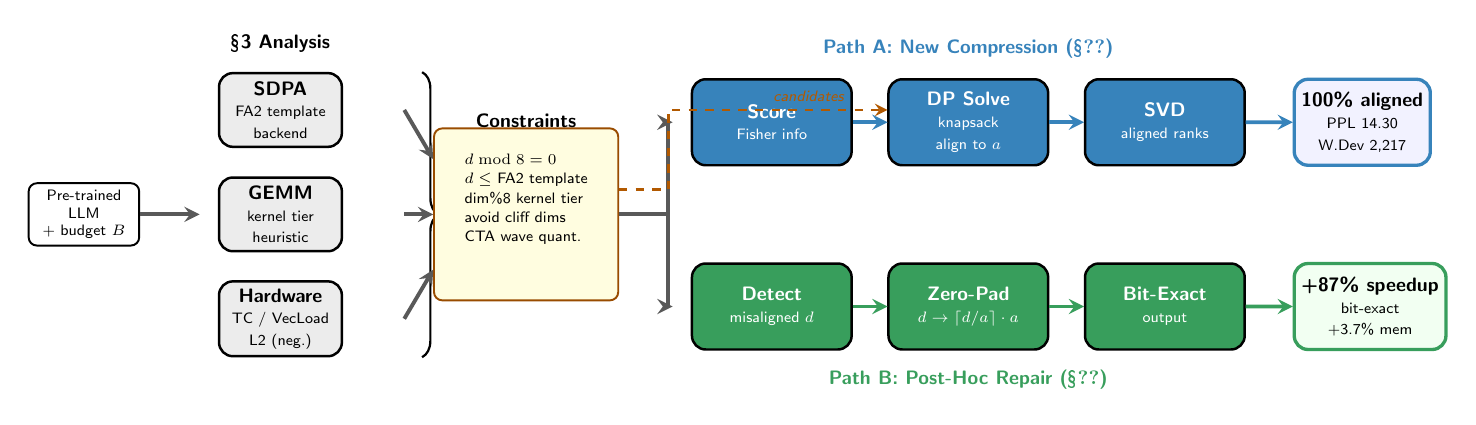
\begin{tikzpicture}[scale=0.78, every node/.style={scale=0.78},
    >=stealth,
    % Colors
    cblue/.style={fill={rgb,255:red,55;green,131;blue,187}},
    cred/.style={fill={rgb,255:red,211;green,63;blue,73}},
    cgreen/.style={fill={rgb,255:red,56;green,158;blue,92}},
    corange/.style={fill={rgb,255:red,230;green,159;blue,0}},
    cgray/.style={fill=gray!15},
    % Box styles
    phase/.style={draw, rounded corners=5pt, minimum width=2.4cm, minimum height=1.6cm,
                  line width=0.9pt, text=white, font=\sffamily\small, align=center},
    constraint/.style={draw, rounded corners=3pt, minimum width=2.0cm, minimum height=0.7cm,
                       line width=0.7pt, font=\sffamily\scriptsize, align=center,
                       fill=yellow!12, draw=orange!60!black},
    result/.style={draw, rounded corners=5pt, minimum width=2.2cm, minimum height=1.6cm,
                   line width=1.2pt, font=\sffamily\small, align=center},
    lbl/.style={font=\sffamily\small, align=center},
    arrow/.style={->, line width=1.4pt, color=gray!70!black},
    dasharrow/.style={->, line width=1.0pt, dashed, color=gray!50},
  ]

  % ===== LEFT: Analysis (§3) =====
  \node[phase, cgray, text=black, minimum width=2.0cm, minimum height=1.2cm]
    (sdpa) at (0, 1.2) {\textbf{SDPA}\\[-1pt]{\scriptsize FA2 template}\\[-1pt]{\scriptsize backend}};
  \node[phase, cgray, text=black, minimum width=2.0cm, minimum height=1.2cm]
    (gemm) at (0, -0.5) {\textbf{GEMM}\\[-1pt]{\scriptsize kernel tier}\\[-1pt]{\scriptsize heuristic}};
  \node[phase, cgray, text=black, minimum width=2.0cm, minimum height=1.2cm]
    (hw) at (0, -2.2) {\textbf{Hardware}\\[-1pt]{\scriptsize TC / VecLoad}\\[-1pt]{\scriptsize L2 (neg.)}};

  % Brace for analysis
  \node[above=0.15cm of sdpa, font=\sffamily\bfseries\small] {\S3 Analysis};
  \draw[decorate, decoration={brace, amplitude=6pt, raise=2pt}, line width=0.8pt]
    ([xshift=1.2cm]sdpa.north east) -- ([xshift=1.2cm]hw.south east);

  % ===== CENTER: Constraints =====
  \node[constraint, minimum width=3.0cm, minimum height=2.8cm]
    (constraints) at (4.0, -0.5) {};
  \node[above=-0.1cm of constraints.north, font=\sffamily\bfseries\small] {Constraints};
  \node[font=\sffamily\scriptsize, align=left, anchor=north] at ([yshift=-0.3cm]constraints.north) {
    $d \bmod 8 = 0$\\[1pt]
    $d \leq$ FA2 template\\[1pt]
    dim\%8 kernel tier\\[1pt]
    avoid cliff dims\\[1pt]
    CTA wave quant.
  };

  % Arrows: analysis → constraints
  \draw[arrow] ([xshift=1.0cm]sdpa.east) -- ([yshift=0.9cm]constraints.west);
  \draw[arrow] ([xshift=1.0cm]gemm.east) -- (constraints.west);
  \draw[arrow] ([xshift=1.0cm]hw.east) -- ([yshift=-0.9cm]constraints.west);

  % ===== RIGHT: Two paths =====
  % Path A: GAC DP (new compression)
  \node[phase, cblue, minimum width=2.6cm, minimum height=1.4cm]
    (score) at (8.0, 1.0) {\textbf{Score}\\[-1pt]{\scriptsize Fisher info}};
  \node[phase, cblue, minimum width=2.6cm, minimum height=1.4cm]
    (dp) at (11.2, 1.0) {\textbf{DP Solve}\\[-1pt]{\scriptsize knapsack}\\[-1pt]{\scriptsize align to $a$}};
  \node[phase, cblue, minimum width=2.6cm, minimum height=1.4cm]
    (svd) at (14.4, 1.0) {\textbf{SVD}\\[-1pt]{\scriptsize aligned ranks}};

  % Path B: Dimension Repair (existing model)
  \node[phase, cgreen, minimum width=2.6cm, minimum height=1.4cm]
    (detect) at (8.0, -2.0) {\textbf{Detect}\\[-1pt]{\scriptsize misaligned $d$}};
  \node[phase, cgreen, minimum width=2.6cm, minimum height=1.4cm]
    (pad) at (11.2, -2.0) {\textbf{Zero-Pad}\\[-1pt]{\scriptsize $d \to \lceil d/a\rceil \cdot a$}};
  \node[phase, cgreen, minimum width=2.6cm, minimum height=1.4cm]
    (exact) at (14.4, -2.0) {\textbf{Bit-Exact}\\[-1pt]{\scriptsize output}};

  % Arrows within paths
  \draw[arrow, color={rgb,255:red,55;green,131;blue,187}] (score) -- (dp);
  \draw[arrow, color={rgb,255:red,55;green,131;blue,187}] (dp) -- (svd);
  \draw[arrow, color={rgb,255:red,56;green,158;blue,92}] (detect) -- (pad);
  \draw[arrow, color={rgb,255:red,56;green,158;blue,92}] (pad) -- (exact);

  % Constraints → paths
  \draw[arrow] (constraints.east) -- ++(0.8,0) |- ([xshift=-0.3cm]score.west)
    node[pos=0.25, above, font=\sffamily\scriptsize\itshape] {};
  \draw[arrow] (constraints.east) -- ++(0.8,0) |- ([xshift=-0.3cm]detect.west);

  % Constraints feeds into DP
  \draw[dasharrow, color=orange!70!black]
    ([yshift=0.4cm]constraints.east) -- ++(0.8,0) |- ([yshift=0.2cm]dp.west)
    node[pos=0.82, above, font=\sffamily\scriptsize\itshape, text=orange!70!black] {candidates};

  % Path labels
  \node[above=0.15cm of dp, font=\sffamily\bfseries\small, text={rgb,255:red,55;green,131;blue,187}]
    {Path A: New Compression (\S\ref{sec:gac})};
  \node[below=0.15cm of pad, font=\sffamily\bfseries\small, text={rgb,255:red,56;green,158;blue,92}]
    {Path B: Post-Hoc Repair (\S\ref{sec:repair})};

  % Results on the right
  \node[result, fill=blue!5, draw={rgb,255:red,55;green,131;blue,187},
        right=0.6cm of svd, minimum height=1.4cm] (resA) {
    {\small\bfseries 100\% aligned}\\[-1pt]
    {\scriptsize PPL 14.30}\\[-1pt]
    {\scriptsize W.Dev 2{,}217}
  };
  \node[result, fill=green!5, draw={rgb,255:red,56;green,158;blue,92},
        right=0.6cm of exact, minimum height=1.4cm] (resB) {
    {\small\bfseries +87\% speedup}\\[-1pt]
    {\scriptsize bit-exact}\\[-1pt]
    {\scriptsize +3.7\% mem}
  };
  \draw[arrow, color={rgb,255:red,55;green,131;blue,187}] (svd) -- (resA);
  \draw[arrow, color={rgb,255:red,56;green,158;blue,92}] (exact) -- (resB);

  % Input on the left
  \node[draw, rounded corners=3pt, fill=white, line width=0.7pt,
        font=\sffamily\scriptsize, align=center, minimum width=1.8cm]
    (input) at (-3.2, -0.5) {Pre-trained\\LLM\\+ budget $B$};
  \draw[arrow] (input) -- ([xshift=-0.3cm]gemm.west |- input);

\end{tikzpicture}
\caption{\textbf{GAC framework overview.}
Analysis (\S\ref{sec:analysis}) extracts alignment constraints from three layers (SDPA, GEMM, hardware).
These constraints drive two complementary solutions:
\emph{Path~A}---alignment-aware rank allocation via multi-choice knapsack DP for new compression;
\emph{Path~B}---zero-padding repair for already-compressed models.
Both paths produce fully-aligned dimensions with no accuracy loss (DP) or bit-exact output preservation (repair).}
\label{fig:gac_framework}
\end{figure*}

\begin{figure*}[t]
\centering
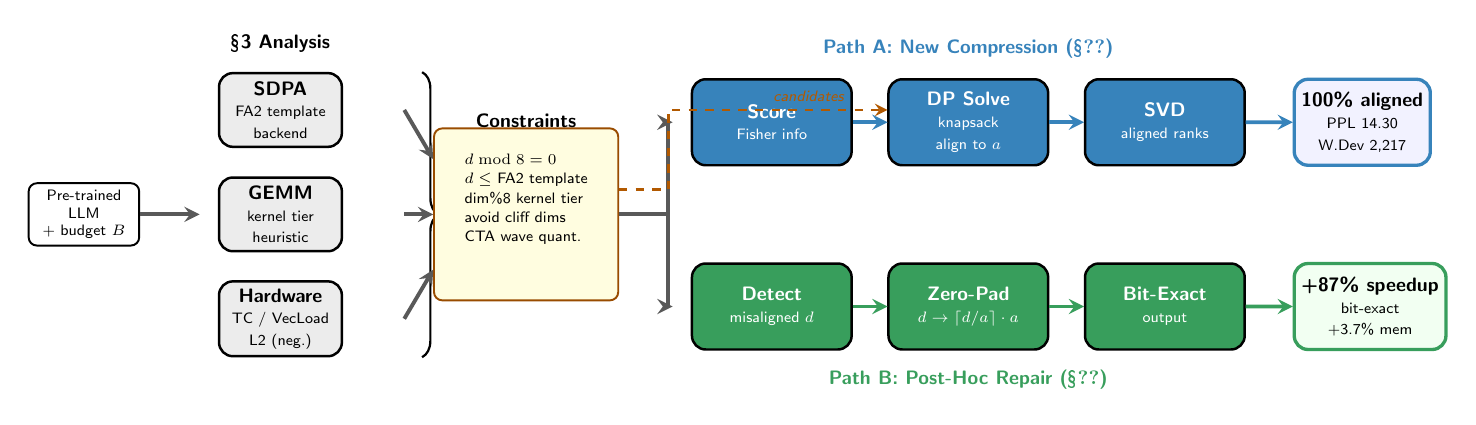
\begin{tikzpicture}[scale=0.78, every node/.style={scale=0.78},
    >=stealth,
    % Colors
    cblue/.style={fill={rgb,255:red,55;green,131;blue,187}},
    cred/.style={fill={rgb,255:red,211;green,63;blue,73}},
    cgreen/.style={fill={rgb,255:red,56;green,158;blue,92}},
    corange/.style={fill={rgb,255:red,230;green,159;blue,0}},
    cgray/.style={fill=gray!15},
    % Box styles
    phase/.style={draw, rounded corners=5pt, minimum width=2.4cm, minimum height=1.6cm,
                  line width=0.9pt, text=white, font=\sffamily\small, align=center},
    constraint/.style={draw, rounded corners=3pt, minimum width=2.0cm, minimum height=0.7cm,
                       line width=0.7pt, font=\sffamily\scriptsize, align=center,
                       fill=yellow!12, draw=orange!60!black},
    result/.style={draw, rounded corners=5pt, minimum width=2.2cm, minimum height=1.6cm,
                   line width=1.2pt, font=\sffamily\small, align=center},
    lbl/.style={font=\sffamily\small, align=center},
    arrow/.style={->, line width=1.4pt, color=gray!70!black},
    dasharrow/.style={->, line width=1.0pt, dashed, color=gray!50},
  ]

  % ===== LEFT: Analysis (§3) =====
  \node[phase, cgray, text=black, minimum width=2.0cm, minimum height=1.2cm]
    (sdpa) at (0, 1.2) {\textbf{SDPA}\\[-1pt]{\scriptsize FA2 template}\\[-1pt]{\scriptsize backend}};
  \node[phase, cgray, text=black, minimum width=2.0cm, minimum height=1.2cm]
    (gemm) at (0, -0.5) {\textbf{GEMM}\\[-1pt]{\scriptsize kernel tier}\\[-1pt]{\scriptsize heuristic}};
  \node[phase, cgray, text=black, minimum width=2.0cm, minimum height=1.2cm]
    (hw) at (0, -2.2) {\textbf{Hardware}\\[-1pt]{\scriptsize TC / VecLoad}\\[-1pt]{\scriptsize L2 (neg.)}};

  % Brace for analysis
  \node[above=0.15cm of sdpa, font=\sffamily\bfseries\small] {\S3 Analysis};
  \draw[decorate, decoration={brace, amplitude=6pt, raise=2pt}, line width=0.8pt]
    ([xshift=1.2cm]sdpa.north east) -- ([xshift=1.2cm]hw.south east);

  % ===== CENTER: Constraints =====
  \node[constraint, minimum width=3.0cm, minimum height=2.8cm]
    (constraints) at (4.0, -0.5) {};
  \node[above=-0.1cm of constraints.north, font=\sffamily\bfseries\small] {Constraints};
  \node[font=\sffamily\scriptsize, align=left, anchor=north] at ([yshift=-0.3cm]constraints.north) {
    $d \bmod 8 = 0$\\[1pt]
    $d \leq$ FA2 template\\[1pt]
    dim\%8 kernel tier\\[1pt]
    avoid cliff dims\\[1pt]
    CTA wave quant.
  };

  % Arrows: analysis → constraints
  \draw[arrow] ([xshift=1.0cm]sdpa.east) -- ([yshift=0.9cm]constraints.west);
  \draw[arrow] ([xshift=1.0cm]gemm.east) -- (constraints.west);
  \draw[arrow] ([xshift=1.0cm]hw.east) -- ([yshift=-0.9cm]constraints.west);

  % ===== RIGHT: Two paths =====
  % Path A: GAC DP (new compression)
  \node[phase, cblue, minimum width=2.6cm, minimum height=1.4cm]
    (score) at (8.0, 1.0) {\textbf{Score}\\[-1pt]{\scriptsize Fisher info}};
  \node[phase, cblue, minimum width=2.6cm, minimum height=1.4cm]
    (dp) at (11.2, 1.0) {\textbf{DP Solve}\\[-1pt]{\scriptsize knapsack}\\[-1pt]{\scriptsize align to $a$}};
  \node[phase, cblue, minimum width=2.6cm, minimum height=1.4cm]
    (svd) at (14.4, 1.0) {\textbf{SVD}\\[-1pt]{\scriptsize aligned ranks}};

  % Path B: Dimension Repair (existing model)
  \node[phase, cgreen, minimum width=2.6cm, minimum height=1.4cm]
    (detect) at (8.0, -2.0) {\textbf{Detect}\\[-1pt]{\scriptsize misaligned $d$}};
  \node[phase, cgreen, minimum width=2.6cm, minimum height=1.4cm]
    (pad) at (11.2, -2.0) {\textbf{Zero-Pad}\\[-1pt]{\scriptsize $d \to \lceil d/a\rceil \cdot a$}};
  \node[phase, cgreen, minimum width=2.6cm, minimum height=1.4cm]
    (exact) at (14.4, -2.0) {\textbf{Bit-Exact}\\[-1pt]{\scriptsize output}};

  % Arrows within paths
  \draw[arrow, color={rgb,255:red,55;green,131;blue,187}] (score) -- (dp);
  \draw[arrow, color={rgb,255:red,55;green,131;blue,187}] (dp) -- (svd);
  \draw[arrow, color={rgb,255:red,56;green,158;blue,92}] (detect) -- (pad);
  \draw[arrow, color={rgb,255:red,56;green,158;blue,92}] (pad) -- (exact);

  % Constraints → paths
  \draw[arrow] (constraints.east) -- ++(0.8,0) |- ([xshift=-0.3cm]score.west)
    node[pos=0.25, above, font=\sffamily\scriptsize\itshape] {};
  \draw[arrow] (constraints.east) -- ++(0.8,0) |- ([xshift=-0.3cm]detect.west);

  % Constraints feeds into DP
  \draw[dasharrow, color=orange!70!black]
    ([yshift=0.4cm]constraints.east) -- ++(0.8,0) |- ([yshift=0.2cm]dp.west)
    node[pos=0.82, above, font=\sffamily\scriptsize\itshape, text=orange!70!black] {candidates};

  % Path labels
  \node[above=0.15cm of dp, font=\sffamily\bfseries\small, text={rgb,255:red,55;green,131;blue,187}]
    {Path A: New Compression (\S\ref{sec:gac})};
  \node[below=0.15cm of pad, font=\sffamily\bfseries\small, text={rgb,255:red,56;green,158;blue,92}]
    {Path B: Post-Hoc Repair (\S\ref{sec:repair})};

  % Results on the right
  \node[result, fill=blue!5, draw={rgb,255:red,55;green,131;blue,187},
        right=0.6cm of svd, minimum height=1.4cm] (resA) {
    {\small\bfseries 100\% aligned}\\[-1pt]
    {\scriptsize PPL 14.30}\\[-1pt]
    {\scriptsize W.Dev 2{,}217}
  };
  \node[result, fill=green!5, draw={rgb,255:red,56;green,158;blue,92},
        right=0.6cm of exact, minimum height=1.4cm] (resB) {
    {\small\bfseries +87\% speedup}\\[-1pt]
    {\scriptsize bit-exact}\\[-1pt]
    {\scriptsize +3.7\% mem}
  };
  \draw[arrow, color={rgb,255:red,55;green,131;blue,187}] (svd) -- (resA);
  \draw[arrow, color={rgb,255:red,56;green,158;blue,92}] (exact) -- (resB);

  % Input on the left
  \node[draw, rounded corners=3pt, fill=white, line width=0.7pt,
        font=\sffamily\scriptsize, align=center, minimum width=1.8cm]
    (input) at (-3.2, -0.5) {Pre-trained\\LLM\\+ budget $B$};
  \draw[arrow] (input) -- ([xshift=-0.3cm]gemm.west |- input);

\end{tikzpicture}
\caption{\textbf{GAC framework overview.}
Analysis (\S\ref{sec:analysis}) extracts alignment constraints from three layers (SDPA, GEMM, hardware).
These constraints drive two complementary solutions:
\emph{Path~A}---alignment-aware rank allocation via multi-choice knapsack DP for new compression;
\emph{Path~B}---zero-padding repair for already-compressed models.
Both paths produce fully-aligned dimensions with no accuracy loss (DP) or bit-exact output preservation (repair).}
\label{fig:gac_framework}
\end{figure*}

\begin{figure*}[t]
\centering
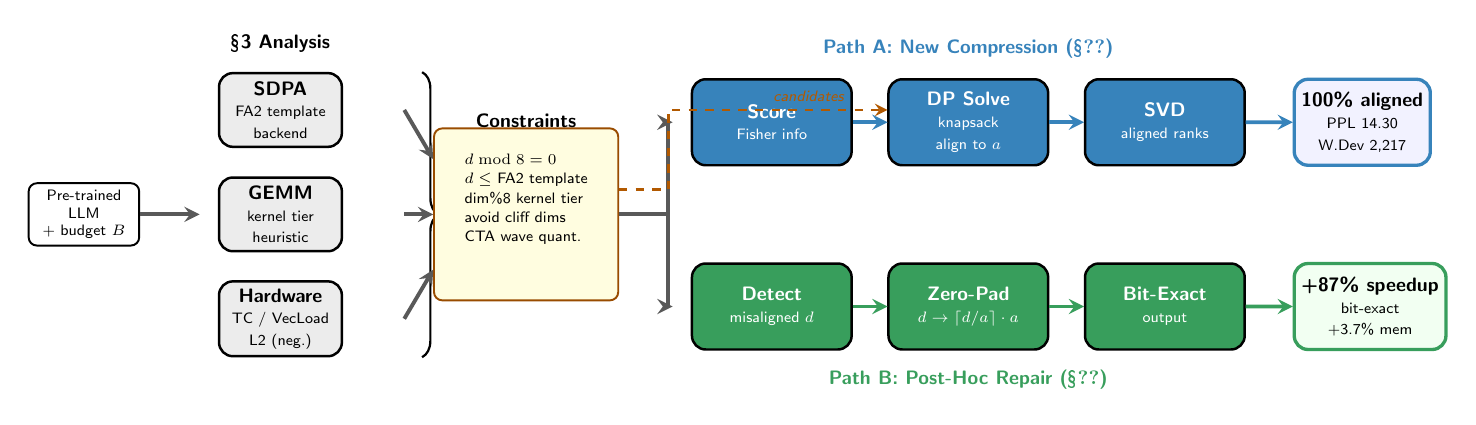
\begin{tikzpicture}[scale=0.78, every node/.style={scale=0.78},
    >=stealth,
    % Colors
    cblue/.style={fill={rgb,255:red,55;green,131;blue,187}},
    cred/.style={fill={rgb,255:red,211;green,63;blue,73}},
    cgreen/.style={fill={rgb,255:red,56;green,158;blue,92}},
    corange/.style={fill={rgb,255:red,230;green,159;blue,0}},
    cgray/.style={fill=gray!15},
    % Box styles
    phase/.style={draw, rounded corners=5pt, minimum width=2.4cm, minimum height=1.6cm,
                  line width=0.9pt, text=white, font=\sffamily\small, align=center},
    constraint/.style={draw, rounded corners=3pt, minimum width=2.0cm, minimum height=0.7cm,
                       line width=0.7pt, font=\sffamily\scriptsize, align=center,
                       fill=yellow!12, draw=orange!60!black},
    result/.style={draw, rounded corners=5pt, minimum width=2.2cm, minimum height=1.6cm,
                   line width=1.2pt, font=\sffamily\small, align=center},
    lbl/.style={font=\sffamily\small, align=center},
    arrow/.style={->, line width=1.4pt, color=gray!70!black},
    dasharrow/.style={->, line width=1.0pt, dashed, color=gray!50},
  ]

  % ===== LEFT: Analysis (§3) =====
  \node[phase, cgray, text=black, minimum width=2.0cm, minimum height=1.2cm]
    (sdpa) at (0, 1.2) {\textbf{SDPA}\\[-1pt]{\scriptsize FA2 template}\\[-1pt]{\scriptsize backend}};
  \node[phase, cgray, text=black, minimum width=2.0cm, minimum height=1.2cm]
    (gemm) at (0, -0.5) {\textbf{GEMM}\\[-1pt]{\scriptsize kernel tier}\\[-1pt]{\scriptsize heuristic}};
  \node[phase, cgray, text=black, minimum width=2.0cm, minimum height=1.2cm]
    (hw) at (0, -2.2) {\textbf{Hardware}\\[-1pt]{\scriptsize TC / VecLoad}\\[-1pt]{\scriptsize L2 (neg.)}};

  % Brace for analysis
  \node[above=0.15cm of sdpa, font=\sffamily\bfseries\small] {\S3 Analysis};
  \draw[decorate, decoration={brace, amplitude=6pt, raise=2pt}, line width=0.8pt]
    ([xshift=1.2cm]sdpa.north east) -- ([xshift=1.2cm]hw.south east);

  % ===== CENTER: Constraints =====
  \node[constraint, minimum width=3.0cm, minimum height=2.8cm]
    (constraints) at (4.0, -0.5) {};
  \node[above=-0.1cm of constraints.north, font=\sffamily\bfseries\small] {Constraints};
  \node[font=\sffamily\scriptsize, align=left, anchor=north] at ([yshift=-0.3cm]constraints.north) {
    $d \bmod 8 = 0$\\[1pt]
    $d \leq$ FA2 template\\[1pt]
    dim\%8 kernel tier\\[1pt]
    avoid cliff dims\\[1pt]
    CTA wave quant.
  };

  % Arrows: analysis → constraints
  \draw[arrow] ([xshift=1.0cm]sdpa.east) -- ([yshift=0.9cm]constraints.west);
  \draw[arrow] ([xshift=1.0cm]gemm.east) -- (constraints.west);
  \draw[arrow] ([xshift=1.0cm]hw.east) -- ([yshift=-0.9cm]constraints.west);

  % ===== RIGHT: Two paths =====
  % Path A: GAC DP (new compression)
  \node[phase, cblue, minimum width=2.6cm, minimum height=1.4cm]
    (score) at (8.0, 1.0) {\textbf{Score}\\[-1pt]{\scriptsize Fisher info}};
  \node[phase, cblue, minimum width=2.6cm, minimum height=1.4cm]
    (dp) at (11.2, 1.0) {\textbf{DP Solve}\\[-1pt]{\scriptsize knapsack}\\[-1pt]{\scriptsize align to $a$}};
  \node[phase, cblue, minimum width=2.6cm, minimum height=1.4cm]
    (svd) at (14.4, 1.0) {\textbf{SVD}\\[-1pt]{\scriptsize aligned ranks}};

  % Path B: Dimension Repair (existing model)
  \node[phase, cgreen, minimum width=2.6cm, minimum height=1.4cm]
    (detect) at (8.0, -2.0) {\textbf{Detect}\\[-1pt]{\scriptsize misaligned $d$}};
  \node[phase, cgreen, minimum width=2.6cm, minimum height=1.4cm]
    (pad) at (11.2, -2.0) {\textbf{Zero-Pad}\\[-1pt]{\scriptsize $d \to \lceil d/a\rceil \cdot a$}};
  \node[phase, cgreen, minimum width=2.6cm, minimum height=1.4cm]
    (exact) at (14.4, -2.0) {\textbf{Bit-Exact}\\[-1pt]{\scriptsize output}};

  % Arrows within paths
  \draw[arrow, color={rgb,255:red,55;green,131;blue,187}] (score) -- (dp);
  \draw[arrow, color={rgb,255:red,55;green,131;blue,187}] (dp) -- (svd);
  \draw[arrow, color={rgb,255:red,56;green,158;blue,92}] (detect) -- (pad);
  \draw[arrow, color={rgb,255:red,56;green,158;blue,92}] (pad) -- (exact);

  % Constraints → paths
  \draw[arrow] (constraints.east) -- ++(0.8,0) |- ([xshift=-0.3cm]score.west)
    node[pos=0.25, above, font=\sffamily\scriptsize\itshape] {};
  \draw[arrow] (constraints.east) -- ++(0.8,0) |- ([xshift=-0.3cm]detect.west);

  % Constraints feeds into DP
  \draw[dasharrow, color=orange!70!black]
    ([yshift=0.4cm]constraints.east) -- ++(0.8,0) |- ([yshift=0.2cm]dp.west)
    node[pos=0.82, above, font=\sffamily\scriptsize\itshape, text=orange!70!black] {candidates};

  % Path labels
  \node[above=0.15cm of dp, font=\sffamily\bfseries\small, text={rgb,255:red,55;green,131;blue,187}]
    {Path A: New Compression (\S\ref{sec:gac})};
  \node[below=0.15cm of pad, font=\sffamily\bfseries\small, text={rgb,255:red,56;green,158;blue,92}]
    {Path B: Post-Hoc Repair (\S\ref{sec:repair})};

  % Results on the right
  \node[result, fill=blue!5, draw={rgb,255:red,55;green,131;blue,187},
        right=0.6cm of svd, minimum height=1.4cm] (resA) {
    {\small\bfseries 100\% aligned}\\[-1pt]
    {\scriptsize PPL 14.30}\\[-1pt]
    {\scriptsize W.Dev 2{,}217}
  };
  \node[result, fill=green!5, draw={rgb,255:red,56;green,158;blue,92},
        right=0.6cm of exact, minimum height=1.4cm] (resB) {
    {\small\bfseries +87\% speedup}\\[-1pt]
    {\scriptsize bit-exact}\\[-1pt]
    {\scriptsize +3.7\% mem}
  };
  \draw[arrow, color={rgb,255:red,55;green,131;blue,187}] (svd) -- (resA);
  \draw[arrow, color={rgb,255:red,56;green,158;blue,92}] (exact) -- (resB);

  % Input on the left
  \node[draw, rounded corners=3pt, fill=white, line width=0.7pt,
        font=\sffamily\scriptsize, align=center, minimum width=1.8cm]
    (input) at (-3.2, -0.5) {Pre-trained\\LLM\\+ budget $B$};
  \draw[arrow] (input) -- ([xshift=-0.3cm]gemm.west |- input);

\end{tikzpicture}
\caption{\textbf{GAC framework overview.}
Analysis (\S\ref{sec:analysis}) extracts alignment constraints from three layers (SDPA, GEMM, hardware).
These constraints drive two complementary solutions:
\emph{Path~A}---alignment-aware rank allocation via multi-choice knapsack DP for new compression;
\emph{Path~B}---zero-padding repair for already-compressed models.
Both paths produce fully-aligned dimensions with no accuracy loss (DP) or bit-exact output preservation (repair).}
\label{fig:gac_framework}
\end{figure*}


\subsection{Overview}

GAC operates as a post-processing wrapper around any existing compressor, adding alignment awareness in three steps (Figure~\ref{fig:gac_framework}):
\textbf{(1)~Operator Analysis}---profile SDPA and GEMM to identify alignment constraints and performance cliffs (\S\ref{sec:analysis});
\textbf{(2)~Dimension Sweep}---sweep dimensions near each ideal rank to build a per-projection candidate table of hardware-friendly values;
\textbf{(3)~Constrained Optimization}---solve a multi-choice knapsack DP to select one candidate per projection, maximizing information preservation under the total parameter budget.

\subsection{Problem Formulation}

Given $n$ projections with Fisher scores $\{f_i\}$, ideal (unconstrained) ranks $\{r_i^*\}$, and total parameter budget $B$, we seek aligned allocations $\{r_i\}$ that maximize Fisher-weighted information preservation:
\begin{equation}
\max_{\{r_i\}} \sum_{i=1}^{n} f_i \cdot (r_i - r_i^*) \;\;\text{s.t.}\;\; \sum_{i} r_i \cdot g_i \leq B,\;\; r_i \in C_i
\label{eq:gac}
\end{equation}
where $g_i$ is the group size for projection $i$ and $C_i$ is the set of hardware-friendly candidates.
The objective is \emph{asymmetric}: rounding up ($r_i > r_i^*$) yields positive value (information preserved), while rounding down yields negative value (information lost), weighted by each layer's Fisher score.
High-Fisher (sensitive) layers naturally receive more rank; low-Fisher (insensitive) layers absorb the cost.

\subsection{Candidate Generation via Dimension Sweep}

Rather than hard-coding alignment to fixed multiples (e.g., mod~8 or mod~32), GAC generates candidates empirically.
For each projection, we profile GEMM and SDPA latency at dimensions near $r_i^*$ and retain only those that avoid performance cliffs.
This produces $|C_i| \approx 11$--$17$ candidates per projection.
Cliff dimensions---where cuBLAS switches kernel tier or SDPA falls back---are automatically excluded.
For example, given an ideal rank $r^*{=}107.3$, the sweep produces $C{=}\{96, 104, 112, 128\}$, excluding 107 because it triggers a cuBLAS performance cliff; the DP then picks $r{=}104$, saving budget for more sensitive layers.
Because the sweep is hardware-specific, GAC adapts to different GPU architectures without manual tuning.

\subsection{Multi-Choice Knapsack DP}

We solve Eq.~\ref{eq:gac} via dynamic programming.
For each candidate $r_{ij} \in C_i$, define value $v_{ij} = f_i \cdot (r_{ij} - r_i^*)$ and weight $w_{ij} = r_{ij} \cdot g_i$.
The DP recurrence is:
\[
D[i][b] = \max_{j} \left\{ D[i{-}1][b - w_{ij}] + v_{ij} \right\}
\]
Complexity: $O(n \cdot |C| \cdot B')$ where $B' = B/(a \cdot g)$ is the quantized budget.
In practice, with $n$=224 projections and $|C|$$\approx$15, the DP runs in under one second on CPU.

Figure~\ref{fig:alg_gac} gives the complete procedure.

\begin{figure}[t]
\centering
\rule{\columnwidth}{0.5pt}
\begin{minipage}{0.94\columnwidth}\small
\textbf{Algorithm:} GAC --- GPU-Aligned Compression\\[2pt]
\textbf{Input:} Pre-trained LLM, compressor, budget $B$\\
\textbf{Output:} Aligned ranks $\{r_i\}_{i=1}^n$ with $r_i \in C_i$\\[2pt]
\rule{\linewidth}{0.3pt}\\[2pt]
\textit{Phase 1: Compressor \& Analysis}\\[1pt]
\hspace*{1em}1.\; Run compressor $\to$ ideal ranks $\{r_i^*\}$, Fisher $\{f_i\}$\\
\hspace*{1em}2.\; Profile GEMM/SDPA $\to$ constraints (\S\ref{sec:analysis})\\[3pt]
\textit{Phase 2: Candidate Generation}\\[1pt]
\hspace*{1em}3.\; \textbf{for} each projection $i = 1, \ldots, n$ \textbf{do}\\
\hspace*{2.5em}Sweep dims near $r_i^*$; measure latency\\
\hspace*{2.5em}$C_i \gets$ dims avoiding perf.\ cliffs\\[3pt]
\textit{Phase 3: Multi-Choice Knapsack DP}\\[1pt]
\hspace*{1em}4.\; $B' \gets B / (a \cdot g)$\\
\hspace*{1em}5.\; $D[0..n][0..B'] \gets -\infty$;\; $D[0][0] \gets 0$\\
\hspace*{1em}6.\; \textbf{for} $i = 1$ to $n$ \textbf{do}\\
\hspace*{2.5em}\textbf{for} each $r_{ij} \in C_i$ \textbf{do}\\
\hspace*{4em}$v_{ij} \gets f_i \cdot (r_{ij} {-} r_i^*)$;\;
             $w_{ij} \gets r_{ij} \cdot g_i$\\
\hspace*{4em}\textbf{for} $b = w_{ij}$ to $B'$ \textbf{do}\\
\hspace*{5.5em}$D[i][b] \gets \max\!\bigl(D[i][b],\;$\\
\hspace*{8em}$D[i{-}1][b{-}w_{ij}] + v_{ij}\bigr)$\\
\hspace*{1em}7.\; Backtrack from $\arg\max_b D[n][b]$\\
\hspace*{1em}\textbf{return} $\{r_i\}$
\end{minipage}
\rule{\columnwidth}{0.5pt}
\caption{\textbf{GAC algorithm.} Phase~1 uses any existing compressor; Phase~2 profiles hardware; Phase~3 solves the knapsack in $O(n {\cdot} |C| {\cdot} B')$ time ($<$1\,s on CPU for $n$=224).}
\label{fig:alg_gac}
\end{figure}


%% ===========================================
%% 5. EVALUATION
%% ===========================================
\section{Evaluation}
\label{sec:eval}

\subsection{Setup}

\paragraph{Model and hardware.}
Llama-3-8B~\cite{llama3} (8.03B parameters) on NVIDIA A100 80GB, PyTorch 2.9.1, CUDA 12.8.
All latency is prefill (compute-bound GEMM); we focus on prefill because it is where alignment most affects performance.

\paragraph{Compression methods.}
We evaluate two representative methods that change tensor dimensions in orthogonal ways:
\textbf{(1)~ASVD}~\cite{asvd}: Activation-aware SVD factorization applied to all 224 attention and MLP projections, compressing 15\% of parameters.
Each weight $W$ is decomposed into $A \cdot B$ where the inner dimension (rank) $r$ is allocated based on PPL-calibrated sensitivity.
\textbf{(2)~LLM-Pruner}~\cite{llmpruner}: Coupled structured pruning of MLP intermediate dimensions across 28 of 32 layers, removing 15\% of parameters.
Each layer's intermediate dimension is reduced independently based on importance.

\paragraph{Strategies.}
For each compressor: \emph{Unaligned} (default output with irregular dimensions) and \emph{GAC} (dimensions aligned to multiples of 8).

\paragraph{Metrics.}
Alignment (\% of projections where $d \bmod 8 = 0$), perplexity (WikiText-2, 2048-token blocks), accuracy (average of PIQA and HellaSwag zero-shot), and prefill latency ($S$=1024, batch=1, 30 measurements after warmup).

\subsection{Main Results}

Table~\ref{tab:main_results} presents the end-to-end comparison.

\begin{table}[t]
\centering
\caption{\textbf{Main results} on Llama-3-8B (15\% compression, A100 80GB). Prefill latency at sequence length 1024. Percentages are relative to baseline.}
\label{tab:main_results}
\small
\setlength{\tabcolsep}{3pt}
\begin{tabular}{@{}lcrcc@{}}
\toprule
\textbf{Method} & \textbf{Align} & \textbf{PPL}$\downarrow$ & \textbf{Acc} & \textbf{Prefill (ms)} \\
\midrule
\rowcolor{gray!10} Baseline & 100\% & 6.14 & 0.72 & 99.6 \\
\midrule
ASVD (Unaln.) & 5\% & 34.7 & 0.38 & 100.5\,{\scriptsize\textcolor{cred}{+1\%}} \\
ASVD (GAC) & 100\% & \textbf{31.3} & 0.39 & \textbf{67.1}\,{\scriptsize\textcolor{cgreen}{$-$33\%}} \\
\midrule
Pruner (Unaln.) & 83\% & 9.88 & 0.67 & 137.7\,{\scriptsize\textcolor{cred}{+38\%}} \\
Pruner (GAC) & 100\% & \textbf{9.87} & 0.67 & \textbf{88.0}\,{\scriptsize\textcolor{cgreen}{$-$12\%}} \\
\bottomrule
\end{tabular}
\end{table}

\paragraph{ASVD: SVD factorization.}
The unconstrained allocation produces 95\% misaligned ranks.
Despite reducing parameters by 15\%, the misaligned model shows \emph{no prefill speedup} (100.5\,ms vs 99.6\,ms baseline)---the compression benefit is entirely consumed by alignment overhead.
GAC restores alignment to 100\%, yielding a 1.5$\times$ prefill speedup (67.1\,ms, $-$33\% vs baseline).
Notably, GAC also improves perplexity (31.3 vs 34.7) because the DP rounds sensitive layers \emph{up}, preserving information where it matters most.

\paragraph{LLM-Pruner: structured pruning.}
The pruned model retains 83\% alignment (most MLP dimensions happen to be near multiples of 8), yet still suffers a +38\% prefill penalty---demonstrating that even partial misalignment triggers significant overhead.
GAC eliminates the penalty entirely, achieving a net 12\% speedup over the uncompressed baseline.
Quality is preserved: PPL and accuracy are nearly identical between Unaligned and GAC variants.

\paragraph{Rank allocation visualization.}
Figure~\ref{fig:gac_ranks} shows per-layer rank allocations for $W_K$ and $W_V$ projections under three strategies.
For $W_K$ (top), GAC DP deviates from both Unaligned and Round-to-8: it rounds \emph{up} for high-Fisher layers (e.g., layers 14--16) and rounds down for insensitive ones, exploiting the asymmetric objective.
For $W_V$ (bottom), most layers retain the full rank (512), with GAC maintaining alignment at the few compressed layers (18--26).

\begin{figure}[t]
\centering
\includegraphics[width=\columnwidth]{figures/fig_gac_ranks.pdf}
\caption{Per-layer rank allocation for $W_K$ (top) and $W_V$ (bottom) projections. GAC DP (blue) deviates from na\"ive rounding (orange) by allocating more rank to sensitive layers.}
\label{fig:gac_ranks}
\end{figure}

\subsection{Prefill Latency Scaling}

The alignment penalty grows with sequence length.
Figure~\ref{fig:prefill_scaling} shows LLM-Pruner prefill latency at four sequence lengths for the three configurations.

\begin{figure}[t]
\centering
\includegraphics[width=\columnwidth]{figures/fig_prefill_scaling.pdf}
\caption{LLM-Pruner prefill latency scaling. The misalignment penalty (red vs.\ gray) grows from +19\% at $S{=}128$ to +38\% at $S{=}1024$ as GEMMs become increasingly compute-bound. GAC (green) consistently matches or beats the uncompressed baseline.}
\label{fig:prefill_scaling}
\end{figure}

The penalty grows from +19\% ($S{=}128$) to +38\% ($S{=}1024$): longer sequences push GEMMs deeper into the compute-bound regime, where Tensor Core utilization and thus alignment dominate.
At $S{=}128$ the model is still partially memory-bound, hiding some misalignment cost; by $S{=}1024$ the penalty is fully exposed.
GAC maintains ${\sim}$12\% speedup over the \emph{uncompressed} baseline for $S \geq 256$, showing that aligned compression delivers both smaller models and faster inference.

\subsection{Discussion}

\paragraph{Why compression does not always speed up inference.}
ASVD decomposes each weight $W$ into two smaller matrices $A$ and $B$, halving FLOPs per projection but doubling the number of GEMM calls.
When ranks are misaligned, each GEMM triggers Tier~2/3 kernels with lower throughput, negating the FLOP reduction entirely---hence the +1\% ``speedup'' of unaligned ASVD.
LLM-Pruner reduces MLP intermediate dimensions but produces sizes like 5931, 6054, and 6778, which fall outside cuBLAS's optimal kernel range.
Even the 83\% naturally-aligned dimensions cannot prevent the +38\% penalty because the remaining 17\% misaligned layers dominate the critical path.

\paragraph{Why prefill but not decode?}
Autoregressive decode uses GeMV ($M{=}1$), which is memory-bound.
As shown in \S\ref{sec:gemv}, GeMV exhibits only ${\sim}$14\% latency variation with no mod-8 pattern---cuBLAS selects memory-optimized kernels that internally pad dimensions.
Alignment matters primarily in the compute-bound prefill regime where Tensor Core utilization limits throughput.

\paragraph{Quantization.}
GPTQ~\cite{gptq} and AWQ~\cite{awq} compress via reduced numerical precision, preserving tensor shapes and naturally avoiding dimensional misalignment.
GAC targets the complementary axis of \emph{dimension-altering} compression (SVD, pruning, KV eviction).
The two compose: first GAC-aligned rank reduction, then quantization, for multiplicative compression.

\paragraph{GAC as a general paradigm.}
GAC operates at \emph{compression time}, requiring no runtime overhead, no architecture changes, and no extra memory---the DP runs in $<$1\,s on CPU.
The dimension sweep is hardware-specific: on A100, it identifies cliffs at SDPA template boundaries and cuBLAS kernel transitions; on H100 with TMA and FA3~\cite{flashattention3}, the cliffs shift accordingly.
For compression libraries, GAC adds negligible computation as a post-processing pass; for serving systems, it eliminates the need for runtime padding (TensorRT~\cite{tensorrt}) or dimension rejection (vLLM~\cite{vllm}).


%% ===========================================
%% 6. RELATED WORK
%% ===========================================
\section{Related Work}
\label{sec:related}

\paragraph{Mainstream compression is hardware-agnostic.}
SVD methods~\cite{asvd,svdllm2024,palu,fwsvd2022,gfwsvd2025} produce irregular ranks without dimensional constraints.
Quantization~\cite{gptq,awq} preserves dimensions via fixed-width groups, naturally avoiding dimensional misalignment.
Pruning~\cite{sparsegpt,wanda,llmpruner} and KV cache compression~\cite{h2o,quest,pyramidkv} may alter dimensions but do not consider hardware alignment.
All target memory reduction; none address GPU performance cliffs caused by irregular dimensions.

\paragraph{Existing hardware-aware approaches fail to address the root cause.}
HALP~\cite{halp2021} formulates CNN pruning as latency-budgeted optimization using end-to-end timing.
HALOC~\cite{haloc2023} uses a differentiable latency prediction model for CNN low-rank compression.
Both are tied to specific compression methods and model families, provide no guarantee on compression ratio, and do not understand the hardware root cause---they measure aggregate latency without isolating dimensional misalignment.
GAC is a general paradigm that wraps any compressor, guarantees the parameter budget, and prevents misalignment via dimension-level root-cause analysis.

\paragraph{Compilers can only react, not prevent.}
Serving systems handle misalignment reactively: FlashAttention-2 pads to the next template ($\sim$30\% overhead); vLLM~\cite{vllm} rejects unsupported \texttt{head\_dim} entirely; TensorRT~\cite{tensorrt} applies runtime padding.
These mitigations waste memory and compute but cannot change model architecture.
Alignment requirements grow stricter across GPU generations~\cite{nvidia_tensor_core_evolution2024}: Hopper introduces TMA with 128-byte transfers~\cite{nvidia_hopper_whitepaper}; FlashAttention-3~\cite{flashattention3} \emph{removes} support for \texttt{head\_dim} 96 and 112.
GAC prevents misalignment at compression time, eliminating the need for runtime workarounds.


%% ===========================================
%% 7. LIMITATIONS AND FUTURE WORK
%% ===========================================
\section{Future Work}
\label{sec:limitations}

All benchmarks are conducted on A100 with FlashAttention-2; newer architectures (H100, Blackwell) impose stricter alignment constraints (TMA descriptors, FP8 Tensor Cores) that may amplify the penalties we observe.
The current GAC prototype operates as an offline post-processing pass rather than an integrated compression framework: it reads a compressed checkpoint, re-allocates ranks via DP, and writes a new checkpoint.
A production-ready implementation should integrate directly into compression libraries so that alignment-aware allocation happens automatically during compression.
We also study SVD and structured pruning in isolation; how alignment constraints interact when multiple techniques are composed (e.g., SVD + GPTQ) remains open.
Finally, GAC redistributes rank budgets without retraining---a lightweight post-GAC finetuning pass could further recover quality at aggressive compression ratios.


%% ===========================================
%% REFERENCES
%% ===========================================
\clearpage
\bibliographystyle{ACM-Reference-Format}
\bibliography{references}


%% ===========================================
%% APPENDIX
%% ===========================================
\appendix

\section{FA2 Template Tiers and Dimension Sweep}
\label{app:fa2_templates}

We sweep \texttt{head\_dim} from 64 to 256 with $B{=}4$, $S{=}2048$, $H{=}32$.
FlashAttention-2 selects the smallest template $t \geq d$; tile width $B_c$ halves at boundaries (e.g., $128 \to 64 \to 32$), so crossing $d{=}128 \to 129$ causes $\sim$90\% latency increase.
Non-8-aligned dimensions trigger the MATH fallback (e.g., $d{=}107$ incurs 2.14\,ms, +40\% vs $d{=}112$ at 1.53\,ms on Flash).
Table~\ref{tab:fa2_templates} quantifies the tiers.

\begin{table}[h]
\centering
\caption{FA2 template tiers and performance ($B{=}4$, $S{=}2048$, $H{=}32$).}
\label{tab:fa2_templates}
\small
\setlength{\tabcolsep}{3pt}
\begin{tabular}{@{}llrrr@{}}
\toprule
Region & Template & $B_r \times B_c$ & Latency & vs.\ $t{=}64$ \\
\midrule
$d{=}64$ & 64 & 128$\times$128 & 0.74\,ms & 1.0$\times$ \\
$d \in (64,96]$ & 96 & 128$\times$64 & 1.12\,ms & 1.5$\times$ \\
$d \in (96,128]$ & 128 & 128$\times$64 & 1.47\,ms & 2.0$\times$ \\
$d \in (128,160]$ & 160 & 128$\times$32 & 2.00\,ms & 2.7$\times$ \\
$d \in (160,256]$ & 192--256 & 128$\times$32 & 2.3--2.9\,ms & 3--4$\times$ \\
\bottomrule
\end{tabular}
\end{table}

\section{Dimension Distribution of Evaluated Methods}
\label{app:dims}

Figure~\ref{fig:dim_distribution} shows the per-layer dimension distributions for ASVD (ranks across 224 projections) and LLM-Pruner (MLP intermediate dimensions across 28 pruned layers).
ASVD ranks range from 300 to 3,185 with 0\% initial alignment; LLM-Pruner dimensions range from 5,931 to 14,336 with 83\% alignment.

\begin{figure*}[h]
\centering
\includegraphics[width=0.85\textwidth]{figures/fig_dim_distribution.pdf}
\caption{Per-layer dimension distributions for ASVD (top) and LLM-Pruner (bottom) on Llama-3-8B with 15\% compression. ASVD: 0\% aligned before GAC; LLM-Pruner: 83\% aligned.}
\label{fig:dim_distribution}
\end{figure*}


\section{Tensor Core Alignment Profiling}
\label{app:tc}

To isolate the Tensor Core misalignment penalty from cuBLAS kernel selection effects, we sweep $K$ and $N$ dimensions at stride 1 near $d$=4096 (the native hidden size of Llama-3-8B) while measuring TFLOPS via Nsight Compute.

Figure~\ref{fig:tc_k_alignment} shows the $K$ dimension sweep.
Aligned values ($K \bmod 16 = 0$) achieve 160--175 TFLOPS, while misaligned values drop to 50--110 TFLOPS---a consistent 50--60\% throughput penalty.
The comb pattern repeats every 16 elements, directly reflecting the \texttt{mma.m16n8k16} tile size.

Figure~\ref{fig:tc_n_alignment} shows the $N$ dimension sweep.
The pattern is similar but with period 8, matching the \texttt{mma.m16n8k16} $N$-tile.
Aligned values ($N \bmod 8 = 0$) reach 155--175 TFLOPS; misaligned values fall to 55--110 TFLOPS.

\begin{figure*}[h]
\centering
\includegraphics[width=0.85\textwidth]{figures/fig_tc_k_alignment.pdf}
\caption{Tensor Core throughput vs.\ $K$ dimension (stride 1 near 4096). Aligned ($K \bmod 16 = 0$) values reach 170+ TFLOPS; misaligned values drop to 50--110 TFLOPS. The comb pattern reflects the \texttt{mma.m16n8k16} tile size.}
\label{fig:tc_k_alignment}
\end{figure*}

\begin{figure*}[h]
\centering
\includegraphics[width=0.85\textwidth]{figures/fig_tc_n_alignment.pdf}
\caption{Tensor Core throughput vs.\ $N$ dimension (stride 1 near 4096). Period-8 comb pattern from $N$-tile of \texttt{mma.m16n8k16}. Misaligned values suffer up to 63\% throughput loss.}
\label{fig:tc_n_alignment}
\end{figure*}


\section{L2 Cache Sector Alignment}
\label{app:l2}

L2 cache operates in 32-byte sectors on A100.
For FP16 data, this corresponds to $K \bmod 16 = 0$ for aligned access.
Figure~\ref{fig:l2_alignment} shows L2 bandwidth as a function of $K$ near 4096.

Aligned values achieve 155--190~GB/s, while misaligned values drop to 70--90~GB/s---a significant raw bandwidth penalty.
However, at the application level (Table~\ref{tab:constraints}), this translates to only ${\sim}$6\% end-to-end impact because cuBLAS internally pads data for its optimized GeMV paths.
This confirms that L2 sector alignment, while measurable in microbenchmarks, is \emph{not} the primary driver of dimensional misalignment.

\begin{figure*}[h]
\centering
\includegraphics[width=0.85\textwidth]{figures/fig_l2_alignment.pdf}
\caption{L2 cache bandwidth vs.\ $K$ dimension. Aligned ($K \bmod 16 = 0$) values achieve 2$\times$ higher bandwidth, but the effect is masked at the application level by cuBLAS internal padding.}
\label{fig:l2_alignment}
\end{figure*}


\section{SVD Rank Distribution Across Compression Ratios}
\label{app:scatter_ratios}

The misalignment problem persists across different compression ratios.
Figure~\ref{fig:scatter_ratios} shows dimension scatter plots for Llama-3-8B under unconstrained SVD allocation at five compression levels ($\rho=0.5$, 0.6, 0.7, 0.8, 0.9) using the Fisher scoring method.
At every ratio, a substantial fraction (40--80\%) of dimensions are misaligned, confirming that dimensional misalignment is inherent to importance-based rank allocation, not an artifact of aggressive compression.

\begin{figure*}[h]
\centering
\begin{subfigure}[t]{\textwidth}
\includegraphics[width=\textwidth]{figures/scatter_1x4_meta_llama_3_8b_instruct_r0.5.pdf}
\caption{Llama-3-8B, $r$=0.5 (50\% compression)}
\end{subfigure}

\vspace{4pt}
\begin{subfigure}[t]{\textwidth}
\includegraphics[width=\textwidth]{figures/scatter_1x4_meta_llama_3_8b_instruct_r0.7.pdf}
\caption{Llama-3-8B, $r$=0.7 (30\% compression)}
\end{subfigure}

\vspace{4pt}
\begin{subfigure}[t]{\textwidth}
\includegraphics[width=\textwidth]{figures/scatter_1x4_meta_llama_3_8b_instruct_r0.9.pdf}
\caption{Llama-3-8B, $r$=0.9 (10\% compression)}
\end{subfigure}

\vspace{4pt}
\begin{subfigure}[t]{\textwidth}
\includegraphics[width=\textwidth]{figures/scatter_1x4_mistral_7b_v0_3_r0.8.pdf}
\caption{Mistral-7B, $\rho=0.8$ (cross-model)}
\end{subfigure}
\caption{SVD rank distributions under unconstrained allocation at various compression ratios and models. Each row shows per-layer head dimensions under four scoring methods. Green = 8-aligned; red = misaligned. Misalignment (50--90\%) is pervasive across all ratios, methods, and model architectures.}
\label{fig:scatter_ratios}
\end{figure*}

\end{document}
